% !TEX root = ../thesis.tex
%
\chapter{Introduction}
\label{ch:intro}

% CONTEXT

% GAP

% INNOVATION

% copy from proposal:

Best practices in software development changed dramatically since its origins in the 1950's~\cite{boehm2006view}.
Software engineering in most of the 20th century was largely based on careful planning and specification, therefore also rather slow-paced and inflexible.
Since twenty years, however, these plan-driven development methods have been frustrating many people because the influencing circumstances change more and more rapidly, not least due to the growing importance of the internet~\cite{Williams2003}.
Product features, which were perfectly valid at the time of their envisioning, would become outdated, irrelevant or otherwise undesirable while the feature was still being planned or implemented as a result of this rapidly changing environment -- not to mention features that are in fact not desired by the customers in the first place.
This insight is often not gained until the feature is shipped to the customer.
As a consequence, short release cycles and fast customer feedback have steadily been growing in importance.
These values are emphasized in \acf{CSE}~\cite{Bosch2014}, which adopts and extends the principles from \emph{DevOps} and agile software development~\cite{Fitzgerald2017,fowler2001agile}.

Adopting the core premises of \ac{CSE} is considered to be a gradual process, which is represented by the \emph{Stairway to Heaven}~\cite{Olsson2012} (see~\cref{fig:stairway}).
Starting from classical software development, the next step is agile software development.
This step is followed by continuous integration, in which integration of the developed software is frequently verified by automated builds and tests~\cite[Maintaining Model Integrity, pp.~341~ff.]{evans2004domain}.
An extension of this is continuous deployment, where the software is automatically deployed to production in continuous cycles.
The last step in the Stairway to Heaven is ``Research \& Development as an Experiment System''.
This means that the continuity gained in the previous steps is used for frequently experimenting with the software and deploying new versions in order to develop software that fits the customer's needs best.
Such an experiment system allows for quicker responses to market changes and more accurate estimation of customer needs~\cite{Olsson2012}.

\begin{figure}[ht]
        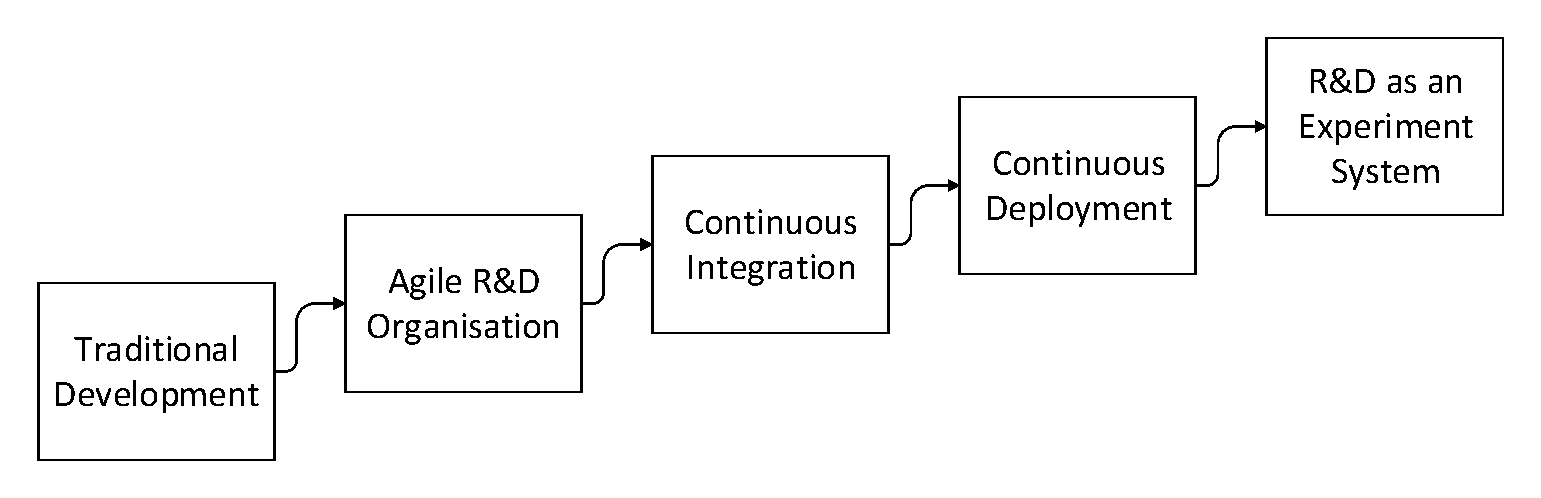
\includegraphics[width=\textwidth]{gfx/stairway.pdf}
        \caption{The ``Stairway to Heaven'' evolutionary model; adapted from~\cite{Olsson2012}.}
        \label{fig:stairway}
\end{figure}

The last step in the Stairway to Heaven requires frequent gathering and analysis of customer feedback, because otherwise an experiment's results could neither be verified nor refuted.
Such feedback may be gathered using active or passive methods.
Active user feedback can yield useful qualitative observations about the product.
The fact that the user has to explicitly take time for giving their feedback, e.g. in form of a survey or an interview, can prove to be problematic in terms of time and effort on both sides.
Passive user feedback, on the other hand, avoids this problem by automatically collecting feedback while the user works with the system as they usually do.
It is thus obtained \emph{implicitly}, hence the equivalent term \emph{implicit user feedback}.
%An example for implicit user feedback is measuring the time a user needs to perform certain actions in the software.

Both approaches for collecting user feedback have their individual advantages and disadvantages.
When experimentation is an integral part of the software engineering process however, the speed and frequency of user feedback becomes more and more important, as \citet{lindgren2015software} have discovered in a study about the state of experimentation in software engineering.
They further state that most techniques which the survey's participants use for feedback gathering are the more familiar \emph{active} techniques, such as stakeholder interviews and usability tests.
Passive techniques are used more rarely and in a less systemic manner, although their advantages are recognized by the survey's participants.
A well-known example for post-deployment passive user feedback collection are A/B tests, where the experiment system automatically reports users' decisions and the variant that they were experiencing.
The results of such an A/B test allow for data-driven decision making about the users' acceptance of a developed feature.
This is opposed to deciding based on active user feedback, which would be too time-consuming to collect in order to allow for a data-driven decision, and an \emph{opinion}-based decision by individuals with stakes in the project.
%, but in software development -- and especially in the post-deployment stage -- most user feedback is collected using passive techniques~\cite{Olsson2014}.

While the overall area of experimentation in software development is well researched, most papers are either more of a report about the state of the art, or a rather abstract description of an architecture.
%This also applies to the paper that initially proposed the Stairway to Heaven concept~\cite{Olsson2012}.
While these reports are very practice-oriented, they lack a more general view on the problem at hand, and the other way around for the more architecture-focused papers.
That is problematic for potential applicants of experimentation techniques in general and \ac{CSE} in particular, because it leaves a gap between theory and current practice.

Therefore, the aim of this thesis is to bridge this gap and provide a more holistic view on collecting, aggregating and analyzing passive user feedback.
%This will enable applicants to implement their own experiment systems as described in \ac{CSE}, based on a proven architecture.
%
%This thesis aims at taking a more holistic approach to the experiment system concept from \ac{CSE} by designing and implementing a system that allows for easy collection of passive user feedback (\cref{sec:intro:goals} describes the objectives in more detail).
The result is a system of interacting services which provide the ability to collect, aggregate and analyze passive user feedback in order to facilitate innovation and experimentation in the research and development process.
%It is anticipated that this system will profit from the usage of event sourcing, especially for its integration into existing experiment systems, but this has to be further investigated in the thesis.
The resulting system shall be called \ac{IFAS}.
It can be adopted by individuals and companies in the software industry who want to fully embrace \ac{CSE} and thus take the last step in the Stairway to Heaven.

\ac{IFAS} utilizes existing software solutions for the different parts of its functionality in order to save both time and effort:
Event Store for data storage, Elasticsearch for aggregating data, and Kibana for visualizing this data for analysis by the \ac{IFAS} user.
The system is implemented as a composition of Docker services and thus available on Linux, Windows, and MacOS.
In its current state, \ac{IFAS} is able to handle about 5,000 events per second and makes them available for analysis in Kibana after usually at most 46.5 seconds.
It facilitates the execution various tasks related to experiment systems, including A/B tests, feature analysis, and monitoring.

%\cite{Bosch2014}

\section{Motivation}
\label{sec:intro:motivation}

% Netflix example
A famous success story for software development with a focus on experimentation -- especially A/B testing -- is that of movie and TV series streaming service Netflix~\cite{WEB:Netflix:2016}.
Big changes such as UI redesigns as well as small ones such as the teaser images for their movies are tested using this platform.
It manages experiments for the whole Netflix platform, which handles 150,000 to 450,000 requests per second (as of 2016), so the experimentation platform is quite elaborate.
From the A/B server that handles, amongst others, the experiment metadata, to the application responsible for the visualization, the presented platform spans at least eight different services.
While this level of complexity is fine and probably needed for an application landscape as big as Netflix', it is not a suitable pattern in terms of cost and complexity for smaller businesses that want to get started with experimentation.
\ac{IFAS} aims to fulfill this need by only using software available without charge and by reducing complexity through omitting service layers which are unnecessary for applications that do not expect such heavy load as Netflix does.

% widening scope of innovation experiments by Bosch2012
Cost is in general a factor when considering the acquisition and commissioning of additional software, and an experiment system -- e.g. \ac{IFAS} -- is no exception.
\citet{Bosch2012} classifies different innovation experiment types as to whether they are suitable for non-commercial deployments or not (cf. \cref{table:intro:motivation:classification}).
According to \citeauthor{Bosch2012}, a product being commercially deployed -- i.e. being profitable or at least expected to be profitable in the near future -- justifies the additional effort and cost to instrument an experiment system for A/B testing and metrics collection in order to improve monetization even more.
These features are A/B testing and collection of (performance) metrics and are available when using \ac{IFAS} due to its functionality.
The fact that \ac{IFAS} is completely free makes these advanced experiments available for non-commercial deployments as well, which is initially not the case according to \citeauthor{Bosch2012}'s classification.
Of course, this is also true for commercial deployments of smaller businesses who do not want to invest in an experiment system yet.
However, there is still some time effort attached to this, and while \ac{IFAS} is designed to be comfortable and time-efficient to use, this is hard to prove and thus such a proof is not attempted in this thesis.

\begin{table}
\centering
\caption[The scope of innovation experiments by \citet{Bosch2012}.]{
The scope of innovation experiments by \citet{Bosch2012}.
\ac{IFAS}' functionality enables A/B testing and collecting metrics (\textit{italic}).
Because the system is free and due to its flexibility, it also potentially enables these for non-commercial deployments.
}
\begin{tabular}{p{2.5cm}|p{3.2cm}|p{3.2cm}|p{3.2cm}}
 & \textbf{Pre-development} & \textbf{Non-commercial deployment} & \textbf{Commercial \newline deployment}  \\ \hline
Optimization & Ethnographic studies & Independently deployed extensions &\textit{ A/B testing}  \\ \hline
New features & Solution jams & Feature alpha & Instrumentation / \textit{collecting metrics}  \\ \hline
New products & Advertising\newline Mockups\newline BASES testing & Product alpha\newline Labs website & Surveys\newline Performance metrics 
\end{tabular}
\label{table:intro:motivation:classification}
\end{table}

% Evolutionary architecture idea
The initial motivation for this thesis was to build an experiment system for evolutionary architectures.
In essence, an evolutionary architecture is an architecture which is designed with future changes in mind~\cite{ford2017building,WEB:EvolArch:2016}.
This is opposed to more traditional approaches where the architecture is designed once and then fixed for the remainder of the project -- or at least only changed very reluctantly because it involves a lot of time and effort.
\ac{IFAS} is designed with the principles of evolutionary architectures in mind, details can be found in \cref{ch:classifications}.
Using event sourcing for the data storage was part of the initial considerations for the system; nevertheless, a proper evaluation of possible alternative data storage solutions was made (cf. \cref{ch:classifications}).

% Most techniques were based on eliciting direct customer feedback through familiar means such as stakeholder interviews and surveys, prototypes, usability and user experience testing, and other forms of user testing. Bug reports and feature voting were also used as a way to guide development. \cite{lindgren2015software}

% Focusing on products and features that create the most customer value was seen as a way to speed up development: ?I don?t think you can accelerate anything. What you can do is do less.? \cite{lindgren2015software}

\section{Objectives}
\label{sec:intro:objectives}

% copy from proposal

The goal of the thesis is to design, implement and validate a system for processing passive user feedback with a more holistic view of the problem than in existing publications.
Using this system, it shall be possible to visualize and analyze passive user feedback that was previously supplied to its storage layer.

In order to accomplish this task, a system with the following functionalities has to be implemented (cf. \cref{fig:system:vision}).
First, a source of the passive user feedback sends data to the \ac{IFAS} storage.
In the planning phase of this thesis, it was not clear whether this user feedback would be generated via usage of a customized web application or an existing data source~\cite{Deka:2017:Rico}.
An evaluation of the data source in question later yielded that it is not suitable for this use case.
The aggregation service in \ac{IFAS} is able to gather relevant data on demand, e.g. using a time- or location-based aggregation.
This data is then displayed in the data analysis application in a visualization of some kind, for example a bar chart or line graph.

The concrete objectives that follow from the desired functionality described until now are as follows:

\begin{enumerate}
\item Classify and choose existing software solutions that implement the needed data storage, aggregation, and analysis functionalities.
\item Design and implement a system that allows the collection of passive user feedback with considerably low effort.
This part of the system is comprised of the storage layer, an aggregation service and a hypothetical client application which logs events to storage whenever the user performs certain actions (cf. 4.).
%It also features two users: The end user of the client application, and the analyst who wants to evaluate the user feedback.
These events can be purely UI related, such as click or hover events, but can also be related to the business logic, like executing transactions or creating content.
In order to forward the user feedback data to the analysis application (cf. 3.), the aggregation service has to fetch the appropriate data from the store.
%While making use of a caching mechanism during this step would certainly make sense, such a feature will presumably not be part of the final solution due to the additional complexity; if this is the case, the system shall be easily extensible for introducing such a feature.
%This objective involves researching and assessing fitting infrastructure and tooling solutions.
\item Design and implement this system such that it also allows analysis of collected user feedback.
Feedback should \emph{usually} be ready for analysis within at most a minute.
When someone wants to evaluate the collected user feedback via the analysis application, the application shall display the corresponding data in an appropriate format, which it fetches from the aggregation service.
The best approach for displaying the data has yet to be evaluated but will involve some graphical representation in form of charts and/or graphs.
%This objective also implicates research and choosing of appropriate solutions that shall be used for this part of the system.
\item Evaluate how this system performs, which involves collecting user feedback and analyzing it.
Implementation of the client application itself will not be done for the purpose of this thesis.
Instead, some existing application shall be extended in order to log the appropriate events or an existing data set such as the one presented by \citet{Deka:2017:Rico} shall be used.
In the latter case, some application or script has to be written which imports the needed UI interaction data to the database.
\item As an additional requirement, the developed system shall be platform independent, i.e. run on the most widely used operating systems Linux, MacOS, and Windows.
\end{enumerate}

\begin{figure}[ht]
        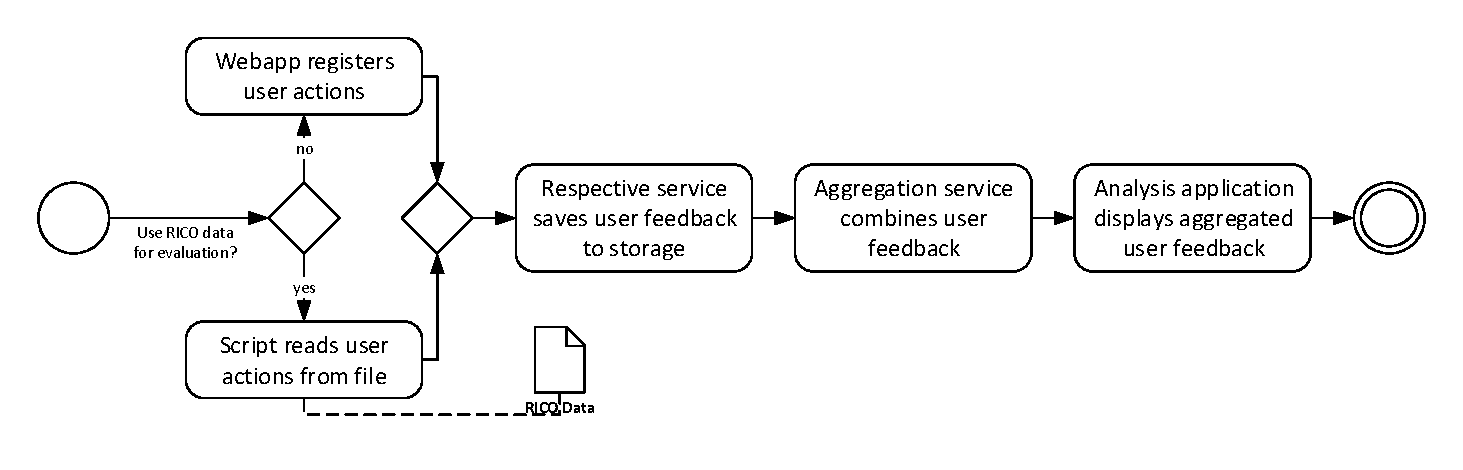
\includegraphics[width=1.1\textwidth]{gfx/architecture-3.pdf}
        \caption{The activities that the envisioned system is able to perform.}
        \label{fig:system:vision}
\end{figure}

%\section{Motivation and Problem Statement}
%\label{sec:intro:motivation}

\section{Thesis Structure}
\label{sec:intro:structure}

In the fundamentals (\cref{ch:fundamentals}), topics that are required to understand the contents of this thesis are explained.
The most important ones are \acf{CSE}, event sourcing, and Docker.

The related work chapter (cf. \cref{ch:related-work}) deals with scientific papers which have already explored the topics of passive user feedback and \ac{CSE} to some degree.

Parts of the research phase were also allotted to researching and comparing appropriate software for the different parts of \ac{IFAS}.
The actual classification and comparison of these solutions is described in \cref{ch:classifications}.
This chapter also includes reasons for the decision against the Rico data source and in favor of a customized web application as well as some considerations regarding container orchestration (cf. \cref{sec:design:data-source,sec:classification:orchestration}).

The actual design and implementation is described in the subsequent \cref{ch:implementation}.
This includes implementation details and general considerations about the client application that connects to \ac{IFAS}, as well as descriptions of the configurations of the various services that make up the main functionality.
Also, an additional bridge application between the storage and aggregation layers was implemented, the need and details of which are represented in \cref{sec:implementation:bridge}.
This chapter also gives a description of the finalized system architecture (cf. \cref{section:design:architecture}).

Finally, the implemented solution was evaluated by executing two experiments (cf. \cref{ch:evaluation}).
The first experiment for the evaluation is a user survey, in which test subjects executed various tasks and afterwards answered several questions about these tasks in a questionnaire (cf. \cref{sec:evaluation:user}).
The results of the questionnaire are compared to the passive user feedback gathered before.
The second experiment tests the performance of \ac{IFAS} in three separate steps, each focusing on a different part of the system (cf. \cref{sec:evaluation:performance}).

Possibilities for future work are given in its own chapter, followed by the conclusion (cf. \cref{ch:future-work,ch:conclusion}).
The appendix at the end of the document contains source code and configuration files of the various applications and services as they are mentioned throughout this thesis.
An enclosed DVD contains the full source code of all implementation work (also available via GitHub\footnote{\url{https://github.com/janis-kra/master-impl}}\todo{link to "final" tag when done}).
The instructions that the test subjects were given during the user survey that was part of the evaluation is attached after the appendix.
